\subsection{Installing the Free Pascal Compiler} % (fold)
\label{sub:installing_fpc}

You can get the Free Pascal Compiler (fpc) for Linux, Mac OS, and Windows. The following section describe where it is you can find these programs, and how to install them.

\subsubsection{Installing fpc on Linux} % (fold)
\label{ssub:fpc_linux}

It should be relatively easy to install \textbf{fpc} for Linux. To install this on Ubuntu linux use the command shown in \lref{lst:apt-get-fpc}.

\bashcode{lst:apt-get-fpc}{The command line instruction to install fpc on Ubuntu}{topics/programs-and-compilers/pascal/apt-get-fpc.txt}

% subsubsection linux (end)

\subsubsection{Installing fpc on Mac OS} % (fold)
\label{ssub:installing_gcc_on_mac_os}

To install \textbf{fpc} on Mac OS you need to install the \textbf{XCode} developer tools, and then the \textbf{Free Pascal Compiler}. You can get the latest version of XCode from the \textbf{Mac App Store}, and then download and install the Free Pascal Compiler from their website.

\begin{itemize}
  \item XCode links:
  \begin{itemize}
    \item Apple's XCode website \url{http://developer.apple.com/xcode/}
    \item Mac App Store  \url{http://itunes.apple.com/au/app/xcode/id448457090?mt=12}
    \item For older version of Mac OS, download from \href{https://developer.apple.com/downloads/download.action?path=Developer_Tools/xcode_3.2.2_developer_tools_beta_20728/xcode322_2148_developerdvd.dmg}{Apple's developer site}.\footnote{These will require you to have an Apple Developer account, which can be done for free at \url{http://developer.apple.com/programs/register}.}
  \end{itemize}
  \item Free Pascal links:
  \begin{itemize}
    \item The Free Pascal Website \url{http://freepascal.org}
    \item Download the compiler from \url{http://sourceforge.net/projects/freepascal/files/} 
  \end{itemize}
\end{itemize}

% subsubsection installing_gcc_on_mac_os (end)

\subsubsection{Installing gcc on Windows} % (fold)
\label{ssub:installing_gcc_on_windows}

To install \textbf{fpc} on Windows you need to install the \textbf{MinGW} program and the \textbf{Free Pascal Compiler}. This includes the MinGW Shell, the Terminal equivalent for Windows. Read the Getting Started page from the links below, and follow the steps for the \textbf{Graphical User Interface Installer}. When following the installer make sure that you choose to install the MinGW Shell as well as the C and C++ compilers.

\begin{itemize}
  \item MinGW:
  \begin{itemize}
    \item The project's Website \url{www.mingw.org}
    \item Instructions for installing MinGW: \url{http://www.mingw.org/wiki/Getting_Started}
    \item Follow the link from the Getting Started article, or download MinGW from Source Forge at \url{http://sourceforge.net/projects/mingw/}
    \item It is a good idea to restart after installing MinGW to make sure all its settings are applied.
  \end{itemize}

  \item Free Pascal links:
  \begin{itemize}
    \item The Free Pascal Website \url{http://freepascal.org}
    \item Download the compiler from \url{http://sourceforge.net/projects/freepascal/files/} 
  \end{itemize}
  
\end{itemize}



% subsubsection installing_gcc_on_windows (end)
% \clearpage
\subsubsection{Testing fpc has installed} % (fold)
\label{ssub:testing_your_install_fpc}

To test that you have successfully installed gcc you can do the following:
\begin{enumerate}
  \item Open a Terminal window. (See the notes on the \nameref{sub:terminal} page for the location of the Terminal program)
  \item At the terminal type \textbf{\texttt{fpc}}. You should see something similar to \fref{fig:fpc-install}. If you see the message `\texttt{-bash: fpc: command not found}' this means the install has not worked correctly. Please review the install steps for your Operating System or get someone to check your install.
\end{enumerate}

\begin{figure}[h]
   \centering
   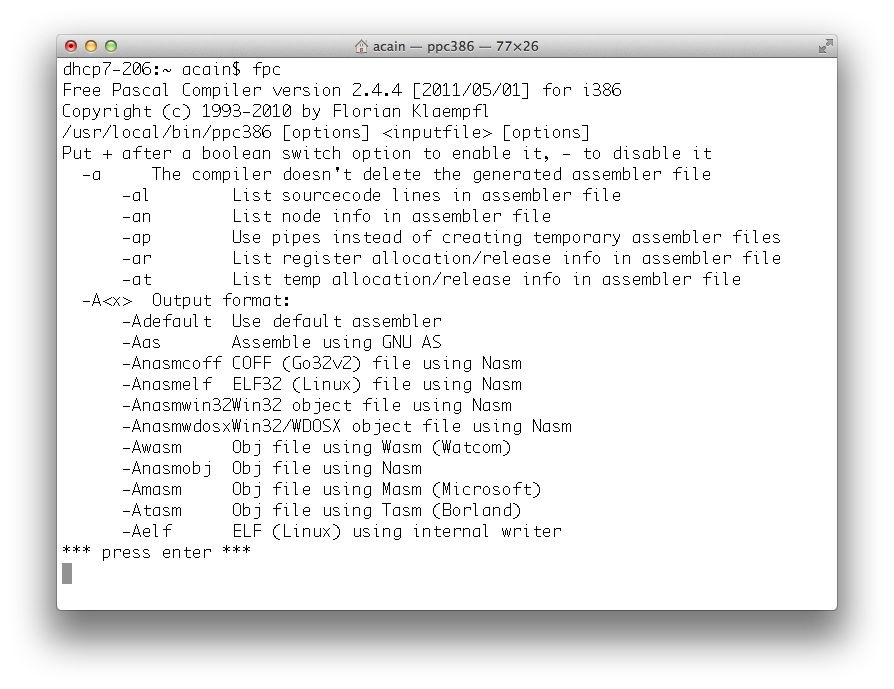
\includegraphics[width=\textwidth]{./topics/programs-and-compilers/images/fpcInstall} 
   \caption{Testing fpc has been installed}
   \label{fig:fpc-install}
\end{figure}

% subsection testing_your_install (end)

% subsection installing_gcc (end)